% 3.4.6 Cumplimiento y transición con el personal (T6).
% Integra la transición con el personal y el estado final del tablero Kanban.

\subsubsection{Cumplimiento y transición con el personal}
\label{sec:ob3_cumplimiento}

Conforme a Kanban, la construcción avanzó con una sola tarjeta en desarrollo y cada tarjeta pasó a «Hecho» solo tras superar sus pruebas. Las dieciséis tarjetas del plan (Tabla~\ref{tab:ob2_tarjetas}) y las cuatro añadidas durante la construcción quedaron completadas (Figura~\ref{fig:ob3_tablero}). El sistema clínico-administrativo quedó en uso en recepción y consultorio, y el agente conversacional, desplegado en el servidor y validado con pacientes simulados en un número dedicado; no se habilitó para los pacientes del centro por las reservas de la clínica sobre el tratamiento de datos en plataformas de terceros, temor que coincide con el principal reporte de odontólogos ecuatorianos \cite{cherrezojeda2020ict}.

\begin{figure}[H]
\centering
\IfFileExists{img/Objetivo3/Ob3_Tablero_Kanban.png}{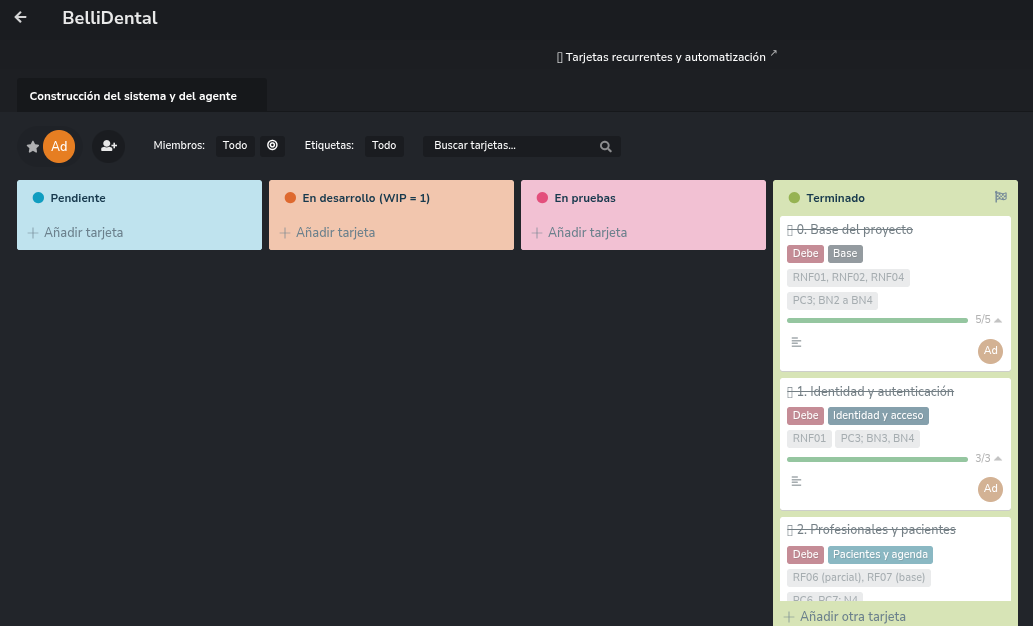
\includegraphics[width=\linewidth]{img/Objetivo3/Ob3_Tablero_Kanban.png}}{\fbox{\parbox{0.9\linewidth}{\centering Pendiente: img/Objetivo3/Ob3\_Tablero\_Kanban.png}}}
\caption{Tablero Kanban con las tarjetas planificadas en estado completado}
\label{fig:ob3_tablero}
\end{figure}
